26. $\cfrac{(x^2-2x-8)(x^2-4x)}{x^2+7x+10}>0\Leftrightarrow\cfrac{x(x-4)^2(x+2)}{(x+2)(x+5)}>0.$ Применив метод интервалов, найдём ответ: $x\in
(-\infty;-5)\cup(0;4)\cup(4;+\infty).$
\begin{figure}[ht!]
\center{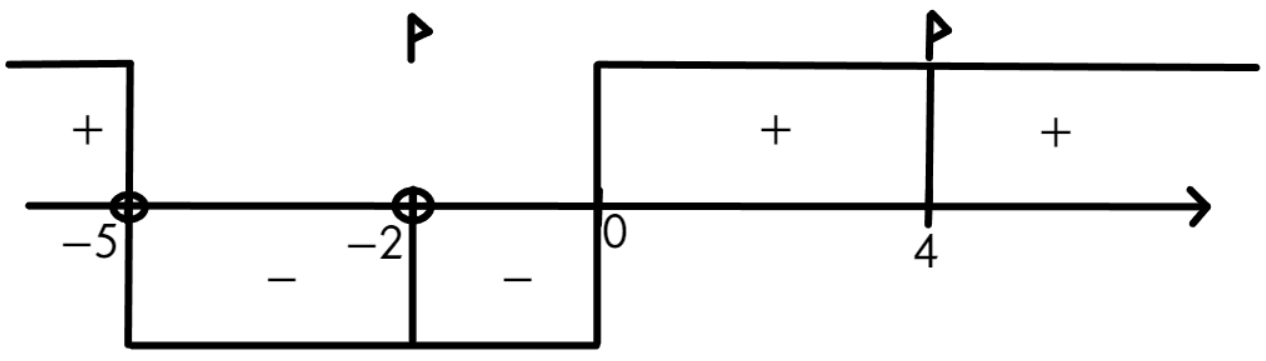
\includegraphics[scale=0.35]{ner9-26.png}}
\end{figure}\\
